\begin{example} Helicoid and catenoid (from homework)

In your homework you have found local parametrizations of helicoid and 
catenoid 
\begin{align*}
    H(u,v)&=\left(v\cos u, v\sin u, a u\right)\\
    C(\varphi,\theta)&=\left(a \cosh \theta \cos \varphi,
    a\cosh \theta \sin \varphi ,a \theta \right) .       
\end{align*}
\begin{figure}[h]
    \centering
    \begin{subfigure}{0.3\textwidth}
        \centering
        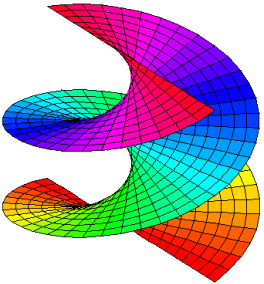
\includegraphics[scale=0.65]{picture/week7/helicoid.png}
        \caption{Helicoid}
    \end{subfigure}
    \begin{subfigure}{0.3\textwidth}
        \centering
        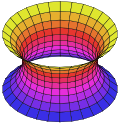
\includegraphics[scale=1.49]{picture/week7/catenoid.png}
        \caption{Catenoid}    
    \end{subfigure}
\end{figure}
\begin{enumerate}[(1)]
    \item Compute the \engordnumber{1} fundamental form of them.
    \[ I_H=\left(v^2+a^2\right)\dd u^2+\dd v^2\]
    \[I_C=\left(a^2\cosh^2\theta\right)\dd\varphi^2+
    \left(a^2\cosh^2\theta\right)\dd \theta^2\]
    \item Show that there is a parametrization on the helicoid, 
    \(\tilde{H}\left(\tilde{u},\tilde{v}\right)\), such that
    \[
        I_{\tilde{H}}=\left(a^2\cosh^2\tilde{v}\right)\dd \tilde{u}^2
        +\left(a^2\cosh^2\tilde{v}^2\right)\dd \tilde{v}^2    
    .\]
    (\(u=\tilde{u},v=a\sinh\tilde{v}\))
\end{enumerate}
\end{example}
\begin{remark}
    In both example 1 and example 3, we have seen that near a point, 
    the two surfaces considered have the same \engordnumber{1} 
    fundamental form
     (after a change of parametrization). Such property is called
      ``local isometry''. We'll make this definition more clear later.
\end{remark}

\(\bullet\)Application of the \engordnumber{1} fundamental form

\begin{enumerate}[(1)]
    \item Arclength of a curve on \(S\).
    
    Note that for a vector \(v\in \mathbb{R}^2\), \(I(v,v)=|v|^2\).
    Let \(\alpha(t)\colon (0,t)\to S\) be a curve in \(S\) and 
    \(\varphi \colon U\to S\), \((u,v)\mapsto\varphi (u,v)\) be a 
    local parametrization satisfying 
    \(\alpha(t)\in \varphi(U)\).
    \[
    \implies \alpha(t)=\varphi\left(u(t),v(t)\right) .   
    \]
    \[
      \implies\alpha'(t)=\varphi_u u'(t)+\varphi_v v'(t) .
    \]
    \[\implies \left|\alpha'(t)\right|^2=
    I\left(\alpha'(t),\alpha'(t)\right)=E u_t^2+2F u_t v_t +G v_t^2.\]
    The arclength of \(\alpha(t)\) is defined by 
    \[
        s(t)=\int_0^t  \left|\alpha'(t)\right|\dd t
        =\int_0^t \sqrt{E u_t^2+2F u_t v_t +G v_t^2}\dd t  .
    \]
    \[
        \implies \dd s=\sqrt{E u_t^2+2F u_t v_t +G v_t^2}\dd t.
    \]
    \[
        \implies\left(\dv{s}{t}\right)^2=E u_t^2+2F u_t v_t +G v_t^2.
    \]
    \[
        \implies \dd s^2=E \dd u^2+2F \dd u \dd v +G \dd v^2    .
    \]
    This explains the ``geometric meaning'' of \(I\), \ie\ it measures 
    the infinitesimal arclength.
    \item Angle between two curves intersecting at \(t_0\).
    
    Let \(\alpha\colon I\to S\), \(\beta\colon I\to S\) be two curves 
    on \(S\), \(\alpha(t_0)=\beta(\bar{t}_0)=p\in S\). 
    \begin{center}
        


\tikzset{every picture/.style={line width=0.75pt}} %set default line width to 0.75pt        

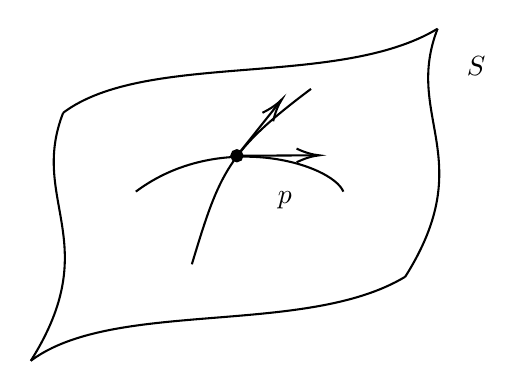
\begin{tikzpicture}[x=0.75pt,y=0.75pt,yscale=-1,xscale=1]
%uncomment if require: \path (0,300); %set diagram left start at 0, and has height of 300

%Curve Lines [id:da9909335153566519] 
\draw    (183,147) .. controls (223,117) and
 (315.4,135.5) .. (363.4,106.5) ;
%Curve Lines [id:da019275275220669075] 
\draw    (167.4,266.5) .. controls (203.4,209.5) and
 (166.4,189.5) .. (183,147) ;
%Curve Lines [id:da6995475257546488] 
\draw    (167.4,266.5) .. controls (207.4,236.5)
 and (299.8,255) .. (347.8,226) ;
%Curve Lines [id:da33316817877336646] 
\draw    (347.8,226) .. controls (383.8,169) and 
(346.8,149) .. (363.4,106.5) ;
%Shape: Circle [id:dp7349369009552857] 
\draw  [fill={rgb, 255:red, 0; green, 0; blue, 0 }  ,fill opacity=1 ] 
(264,167.7) .. controls (264,166.21) and (265.21,165) .. (266.7,165) 
.. controls (268.19,165) and (269.4,166.21) .. (269.4,167.7) .. 
controls (269.4,169.19) and (268.19,170.4) .. (266.7,170.4) .. 
controls (265.21,170.4) and (264,169.19) .. (264,167.7) -- cycle ;
%Curve Lines [id:da09382061994840107] 
\draw    (218,185) .. controls (258,155) and (312.4,171.5) .. (318,185) ;
%Curve Lines [id:da6577705388758515] 
\draw    (245,220) .. controls (258.4,175.5) and (262.4,165.5) .. (302.4,135.5) ;
%Straight Lines [id:da2459893691777446] 
\draw    (266.7,167.7) -- (287.15,142.06) ;
\draw [shift={(288.4,140.5)}, rotate = 128.58] [color={rgb, 255:red, 0; green, 0; blue, 0 }  ]
[line width=0.75]    (10.93,-3.29) .. controls (6.95,-1.4) and (3.31,-0.3) .. (0,0) .. controls 
(3.31,0.3) and (6.95,1.4) .. (10.93,3.29)   ;
%Straight Lines [id:da2821040919294362] 
\draw    (266.7,167.7) -- (304.4,167.51) ;
\draw [shift={(306.4,167.5)}, rotate = 179.71] [color={rgb, 255:red, 0; green, 0; blue, 0 }  ]
[line width=0.75]    (10.93,-3.29) .. controls (6.95,-1.4) and (3.31,-0.3) .. (0,0)
 .. controls (3.31,0.3) 
and (6.95,1.4) .. (10.93,3.29)   ;

% Text Node
\draw (376,118.4) node [anchor=north west][inner sep=0.75pt]    {$S$};
% Text Node
\draw (285,183.4) node [anchor=north west][inner sep=0.75pt]    {$p$};


\end{tikzpicture}
    \end{center}
    Define
        \[
            \cos \theta=\frac{\left\langle\alpha'(t_0),
            \beta'(\bar{t}_0)\right\rangle_{\mathbb{R}^3}}{
            \left|\alpha'(t_0)\right|\left|\beta'(\bar{t}_0) \right|}.
        \]
    \begin{question}
        Given a parametrization \(\varphi(u,v)\),
         we have two coordinate
         curve \(\varphi(u,v_0)\), \(\varphi(u_0,v)\). What's the angle 
         between them?
         \[u\text{-curve: }\alpha(t)=\varphi\left(u(t),c\right)
         \implies \alpha'(t)=\varphi_u u'.\]
         \[v\text{-curve: }\beta(t)=\varphi\left(c,v(t)\right)
         \implies \beta'(t)=\varphi_v v'.\] 
         \[
            \implies \cos \theta= 
            \frac{\left\langle \varphi_u u',\varphi_v v'\right\rangle}{
                \left|\varphi_u u'\right|\left|\varphi_v v'\right|
            }
            =\pm \frac{\left\langle\varphi_u,\varphi_v
            \right\rangle_{\mathbb{R}^3}}{\left|\varphi_u\right|
            \left|\varphi_v\right|}=\pm \frac{F}{\sqrt{EG}}  
         .\]
         In particular, we conclude that
         \[F=0\Leftrightarrow \text{Two coordinate curves are orthogonal,}\]
         and such parametrization is called an orthogonal parametrization.
         (e.g. For \(\mathbb{S}^2\), \((\theta,\varphi)\) and 
         the stereographic projection are two such parametrizations) 
    \end{question}
    \item (Surface) Area.
    
    Let \(S\) be a regular surface. Choose a parametrization 
    \(\varphi\colon U\to S\). Let \(Q\subset S\) be a bounded domain.
    Assume \(Q\subset \varphi(U)\), so \(\varphi^{-1}(Q)\subset U\) is 
    a bounded set in \(\mathbb{R}^2\).
    \begin{center}
\tikzset{every picture/.style={line width=0.75pt}} %set default line width to 0.75pt        

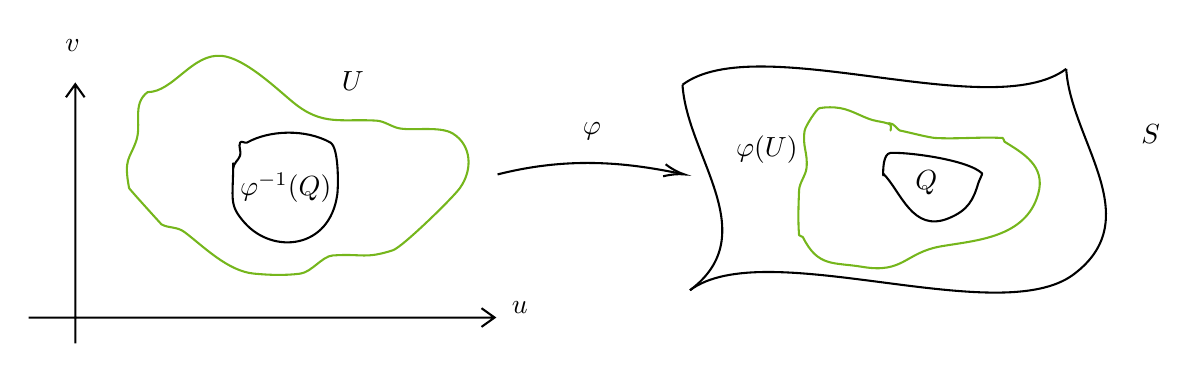
\begin{tikzpicture}[x=0.75pt,y=0.75pt,yscale=-0.9,xscale=0.9]
%uncomment if require: \path (0,300); %set diagram left start at 0, and has height of 300

%Shape: Axis 2D [id:dp30826843172023066] 
\draw  (67,239.62) -- (316.4,239.62)(91.94,114.71) -- (91.94,253.5) (309.4,234.62) -- (316.4,239.62)
 -- (309.4,244.62) (86.94,121.71) -- (91.94,114.71) -- (96.94,121.71)  ;
%Curve Lines [id:da2230443220096674] 
\draw [color={rgb, 255:red, 117; green, 182; blue, 28 }  ,draw opacity=1 ][line width=0.75] 
[line join = round][line cap = round]   (130.65,118.95) .. controls (122.05,125.38) and (127.75,136.1)
.. (124.46,145.32) .. controls (121.04,154.89) and (117.73,154.56) .. (120.74,170.31) .. controls (120.84,170.81) and (138.01,189.7) .. (138.08,189.74) .. controls (142.04,191.95) and (146.26,190.76) .. (150.46,193.9) .. controls (160.22,201.19) and (173.4,214.78) .. (187.61,216.11) .. controls (195.84,216.88) and (204.18,217.17) .. (212.38,216.11) .. controls (218.48,215.32) and (224.1,206.79) .. (229.72,206.39) .. controls (245.72,205.27) and (246.88,208.43) .. (261.91,203.62) .. controls (267,201.99) and (294.17,175.43) .. (297.82,170.31) .. controls (304.87,160.44) and (304.12,147.39) .. (294.11,141.16) .. controls (287.42,136.99) and (273.12,139.67) .. (265.63,138.38) .. controls (261.37,137.65) and (257.55,134.47) .. (253.25,134.22) .. controls (234.05,133.09) and (224.32,137.27) .. (208.67,124.5) .. controls (200.24,117.64) and (182.83,100.69) .. (170.28,99.52) .. controls (154.41,98.04) and (144.45,118.95) .. (130.65,118.95) -- cycle ;
%Curve Lines [id:da779384228982472] 
\draw [line width=0.75] [line join = round][line cap = round]   (176.47,157.04) .. controls (176.47,176.42) and (173.86,179.1) .. (182.66,188.96) .. controls (197.74,205.87) and (228.15,203.16) .. (232.19,173.69) .. controls (232.75,169.62) and (233.14,148.55) .. (228.48,145.93) .. controls (215.25,138.52) and (195.8,139.26) .. (183.9,145.93) .. controls (182.79,146.56) and (180.82,144.74) .. (180.18,145.93) .. controls (179.12,147.92) and (180.91,150.71) .. (180.18,152.87) .. controls (179.34,155.4) and (176.47,157.12) .. (176.47,159.81) ;
%Curve Lines [id:da4093176006038537] 
\draw    (417,115) .. controls (457,85) and (582.4,136.5) .. (622.4,106.5) ;
%Curve Lines [id:da8843839986108935] 
\draw    (421,225) .. controls (461,195) and (586.4,246.5) .. (626.4,216.5) ;
%Curve Lines [id:da3854765584435005] 
\draw    (421,225) .. controls (461,195) and (419.4,153.5) .. (417,115) ;
%Curve Lines [id:da6146348531460317] 
\draw    (626.4,216.5) .. controls (666.4,186.5) and (624.8,145) .. (622.4,106.5) ;
%Curve Lines [id:da8543149552748068] 
\draw [color={rgb, 255:red, 117; green, 182; blue, 28 }  ,draw opacity=1 ][line width=0.75] [line join = round][line cap = round]   (528.4,139.5) .. controls (528.4,138.5) and (528.85,137.39) .. (528.4,136.5) .. controls (527.93,135.57) and (522.09,134.61) .. (521.4,134.5) .. controls (514.38,133.33) and (508.52,128.69) .. (501.4,127.5) .. controls (497.78,126.9) and (494.02,126.9) .. (490.4,127.5) .. controls (488.74,127.78) and (482.76,137.32) .. (482.4,139.5) .. controls (480.99,147.95) and (484.21,151.37) .. (483.4,159.5) .. controls (483,163.53) and (479.56,167.46) .. (479.4,171.5) .. controls (479.09,179.49) and (478.76,187.53) .. (479.4,195.5) .. controls (479.46,196.24) and (481.07,195.83) .. (481.4,196.5) .. controls (489.58,212.86) and (497.61,209.87) .. (513.4,212.5) .. controls (535.53,216.19) and (535.97,204.88) .. (555.4,201.5) .. controls (574.04,198.26) and (600.67,197.05) .. (607.4,173.5) .. controls (611.7,158.44) and (599.25,151.66) .. (589.4,145.5) .. controls (588.77,145.1) and (589.14,143.54) .. (588.4,143.5) .. controls (576.42,142.85) and (564.38,144.11) .. (552.4,143.5) .. controls (548.93,143.32) and (537.92,140.4) .. (533.4,139.5) .. controls (532.08,139.24) and (530.49,135.5) .. (527.4,135.5) ;
%Curve Lines [id:da5437419917187927] 
\draw [line width=0.75] [line join = round][line cap = round]   (524.4,162.5) .. controls (533.93,172.03) and (540,194.41) .. (559.4,186.5) .. controls (570.03,182.17) and (572.69,176.55) .. (575.4,167.5) .. controls (575.66,166.65) and (577.6,162.7) .. (577.4,162.5) .. controls (570.13,155.23) and (537.95,150.97) .. (528.4,151.5) .. controls (524.33,151.73) and (524.4,160.76) .. (524.4,163.5) ;
%Curve Lines [id:da9563040601689965] 
\draw    (318,163) .. controls (358.57,152.71) and (390.12,157.31) .. (416.4,162.67) ;
\draw [shift={(418,163)}, rotate = 191.68] [color={rgb, 255:red, 0; green, 0; blue, 0 }  ][line width=0.75]    (10.93,-3.29) .. controls (6.95,-1.4) and (3.31,-0.3) .. (0,0) .. controls (3.31,0.3) and (6.95,1.4) .. (10.93,3.29)   ;

% Text Node
\draw (178.47,160.44) node [anchor=north west][inner sep=0.75pt]    {$\varphi ^{-1}( Q)$};
% Text Node
\draw (233,106.4) node [anchor=north west][inner sep=0.75pt]    {$U$};
% Text Node
\draw (540,159.4) node [anchor=north west][inner sep=0.75pt]    {$Q$};
% Text Node
\draw (444,140.4) node [anchor=north west][inner sep=0.75pt]    {$\varphi ( U)$};
% Text Node
\draw (661,134.4) node [anchor=north west][inner sep=0.75pt]    {$S$};
% Text Node
\draw (362,133.4) node [anchor=north west][inner sep=0.75pt]    {$\varphi $};
% Text Node
\draw (324,229.4) node [anchor=north west][inner sep=0.75pt]    {$u$};
% Text Node
\draw (85,89.4) node [anchor=north west][inner sep=0.75pt]    {$v$};


\end{tikzpicture}
    \end{center}
    Let's assume the boundary of \(Q\) is a differentiable curve with 
    singularities lying in a measure zero set.
\begin{definition}[Area of \(Q\)]
    \[Area(Q)=\iint_{\varphi(Q)} \left|\varphi_u\wedge 
    \varphi_v \right|\dd u\dd v \quad(\text{double integral in }
    \mathbb{R}^2).\]
    Here, we give the definition in terms of a ``parametrization''. 
    However, the area of \(Q\) is a number only depending on \(Q\)
    itself. We should check that our definition does not depend on 
    the parametrization.
\end{definition}
\textbf{Claim}: 
\textcolor{blue}{\(Area(Q)\) defined above is independent of the
choice of parametrizations.}
\begin{proof} (Left as exercise)

    Let \(\psi(\alpha,\beta)\colon V\to S\) be another parametrization. 
    Let \(H=\psi^{-1}\circ \varphi\) be the change of parametrization,
    \(H(u,v)=(\alpha,\beta)\)\(\implies\varphi =\psi \circ H\).
    We compute \(\iint_{\varphi(Q)} \left|\varphi_u\wedge 
    \varphi_v \right|\dd u\dd v\).

    By chain rule 
    \[
        \begin{pmatrix}
            \varphi_u\\ \varphi_v
        \end{pmatrix}=
        \pdv{(\alpha,\beta)}{(u,v)}\begin{pmatrix}
            \psi_\alpha\\
            \psi_\beta
        \end{pmatrix}    .
    \]
    \begin{align*}
        \implies \varphi_u\wedge\varphi_v&=
        \left(\alpha_u\beta_v\right)\psi_\alpha\wedge\psi_\beta+
        \left(\alpha_v\beta_u\right)\psi_\beta\wedge\psi_\alpha\\
        &=\left(\alpha_u\beta_v-\alpha_v\beta_u\right)
        \psi_\alpha\wedge\psi_\beta\\
        &=\det\left(\pdv{(\alpha,\beta)}{(u,v)}\right)
        \psi_\alpha\wedge\psi_\beta.
    \end{align*}
    \[\implies \left|
        \varphi_u\wedge \varphi_v 
    \right|=\left|\det\left(\pdv{(\alpha,\beta)}{(u,v)}\right)\right|
    \left|\psi_\alpha\wedge\psi_\beta\right|.\]
    
    On the other hand,
    \[
        \begin{pmatrix}
            \dd u\\ \dd v
        \end{pmatrix}
        =\pdv{(u,v)}{(\alpha,\beta)}\begin{pmatrix}
            \dd \alpha\\
            \dd \beta
        \end{pmatrix} .
    \]
    Thus, the change of infinitesimal area element is
    \[
        \dd u\dd v=\left|\dd u\wedge\dd v\right|=
        \left|\det \left(\pdv{(u,v)}{(\alpha,\beta)}\right)\right|
        \left|\dd\alpha\wedge\dd\beta\right|=
        \left|\det \left(\pdv{(u,v)}{(\alpha,\beta)}\right)\right|
        \dd\alpha\dd\beta.
    \]
    \[\implies \left|\varphi_u\wedge \varphi_v \right|
        \dd u\dd v=\left|\psi_\alpha\wedge\psi_\beta\right|\dd \alpha
        \dd \beta.
    \]
    \[\implies \iint \left|\varphi_u\wedge \varphi_v \right|
    \dd u\dd v=\iint \left|\psi_\alpha\wedge\psi_\beta\right|\dd \alpha
    \dd \beta.\]
\end{proof}
\begin{remark}
    By the \engordnumber{1} fundamental form 
    \[
        I=E(\dd u)^2+2F \dd u\dd v+G(\dd v)^2    
    \]
    \[\implies Area=\iint \left|\varphi_u\wedge \varphi_v \right|
    \dd u\dd v=\iint \sqrt{EG-F^2}\dd u\dd v.\]
\end{remark}
\end{enumerate}
\section{Gauss maps and the \texorpdfstring{\engordnumber{2}}{2nd} fundamental form}
\(\bullet\) Gauss maps.
\begin{question}
    \textcolor{blue}{How is a regular surface curved in \(\mathbb{R}^3\)}? 
\end{question}
\underline{\textbf{Recall}}: \(S\subset\mathbb{R}^3\) is an oriented
regular surface. 
\(\implies\) We can choose a unit vector field 
    \begin{align*}
        \vb{n}\colon S&\to \mathbb{S}^2(1)\\
        p&\mapsto \vb{n}_p,
    \end{align*}
is well-defined everywhere on \(S\). Moreover, \(\vb{n}\) is a
differentiable map with its image lying on the unit sphere, and we 
called the map to be the Gauss map. \(\vb{n}\) determines an 
orientation of \(S\).
\begin{center}
    


\tikzset{every picture/.style={line width=0.75pt}} %set default line width to 0.75pt        

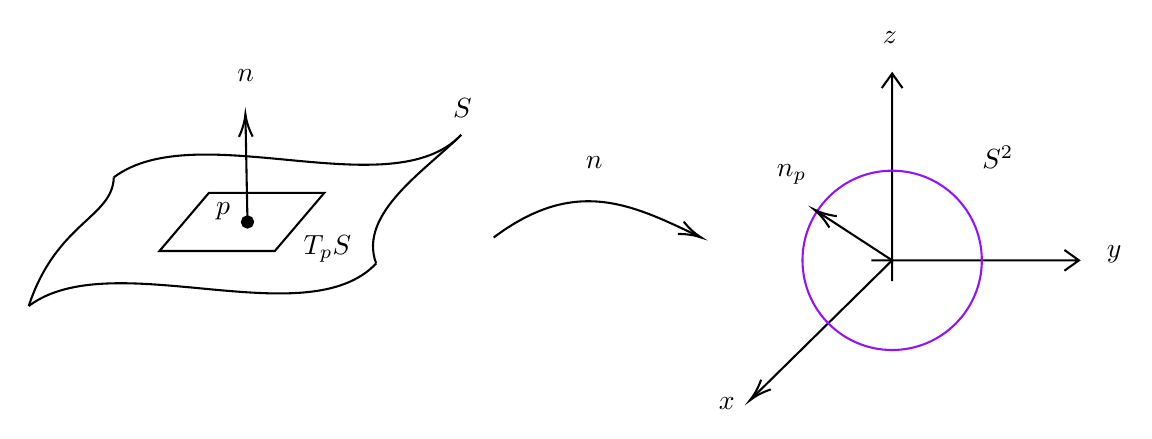
\begin{tikzpicture}[x=0.75pt,y=0.75pt,yscale=-1,xscale=1]
%uncomment if require: \path (0,300); %set diagram left start at 0, and has height of 300

%Curve Lines [id:da28129415507356703] 
\draw    (100,110) .. controls (140,80) and (233.8,125) .. (267.4,89.5) ;
%Curve Lines [id:da9562883564686324] 
\draw    (59,172) .. controls (99,142) and (192.8,187) .. (226.4,151.5) ;
%Curve Lines [id:da748577885122705] 
\draw    (59,172) .. controls (72.4,131.5) and (99.4,129.5) .. (100,110) ;
%Curve Lines [id:da2562375766370064] 
\draw    (226.4,151.5) .. controls (217.4,127.5) and (250.4,106.5) .. (267.4,89.5) ;
%Shape: Parallelogram [id:dp8965230202175429] 
\draw   (145.82,117.5) -- (201.4,117.5) -- (177.58,145.5) -- (122,145.5) -- cycle ;
%Shape: Circle [id:dp3509817579048975] 
\draw  [fill={rgb, 255:red, 0; green, 0; blue, 0 }  ,fill opacity=1 ] (161.7,131.5) .. controls (161.7,130.01) and (162.91,128.8) .. (164.4,128.8) .. controls (165.89,128.8) and (167.1,130.01) .. (167.1,131.5) .. controls (167.1,132.99) and (165.89,134.2) .. (164.4,134.2) .. controls (162.91,134.2) and (161.7,132.99) .. (161.7,131.5) -- cycle ;
%Straight Lines [id:da4477857542457926] 
\draw    (164.4,131.5) -- (163.44,81.5) ;
\draw [shift={(163.4,79.5)}, rotate = 88.9] [color={rgb, 255:red, 0; green, 0; blue, 0 }  ][line width=0.75]    (10.93,-3.29) .. controls (6.95,-1.4) and (3.31,-0.3) .. (0,0) .. controls (3.31,0.3) and (6.95,1.4) .. (10.93,3.29)   ;
%Shape: Axis 2D [id:dp2767501351977306] 
\draw  (465,150) -- (565,150)(475,60) -- (475,160) (558,145) -- (565,150) -- (558,155) (470,67) -- (475,60) -- (480,67)  ;
%Straight Lines [id:da9011328855757925] 
\draw    (475,150) -- (407.83,216.1) ;
\draw [shift={(406.4,217.5)}, rotate = 315.46] [color={rgb, 255:red, 0; green, 0; blue, 0 }  ][line width=0.75]    (10.93,-3.29) .. controls (6.95,-1.4) and (3.31,-0.3) .. (0,0) .. controls (3.31,0.3) and (6.95,1.4) .. (10.93,3.29)   ;
%Shape: Circle [id:dp28714049477405257] 
\draw  [color={rgb, 255:red, 144; green, 19; blue, 254 }  ,draw opacity=1 ] (431.8,150) .. controls (431.8,126.14) and (451.14,106.8) .. (475,106.8) .. controls (498.86,106.8) and (518.2,126.14) .. (518.2,150) .. controls (518.2,173.86) and (498.86,193.2) .. (475,193.2) .. controls (451.14,193.2) and (431.8,173.86) .. (431.8,150) -- cycle ;
%Straight Lines [id:da45439583119974114] 
\draw    (475,150) -- (439.08,126.59) ;
\draw [shift={(437.4,125.5)}, rotate = 33.09] [color={rgb, 255:red, 0; green, 0; blue, 0 }  ][line width=0.75]    (10.93,-3.29) .. controls (6.95,-1.4) and (3.31,-0.3) .. (0,0) .. controls (3.31,0.3) and (6.95,1.4) .. (10.93,3.29)   ;
%Curve Lines [id:da1330380081969107] 
\draw    (283,139) .. controls (322.4,109.45) and (349.58,123.08) .. (381.54,138.3) ;
\draw [shift={(383,139)}, rotate = 205.43] [color={rgb, 255:red, 0; green, 0; blue, 0 }  ][line width=0.75]    (10.93,-3.29) .. controls (6.95,-1.4) and (3.31,-0.3) .. (0,0) .. controls (3.31,0.3) and (6.95,1.4) .. (10.93,3.29)   ;

% Text Node
\draw (190,136.4) node [anchor=north west][inner sep=0.75pt]    {$T_{p} S$};
% Text Node
\draw (158,56.4) node [anchor=north west][inner sep=0.75pt]    {$\vb{n}$};
% Text Node
\draw (147.82,120.9) node [anchor=north west][inner sep=0.75pt]    {$p$};
% Text Node
\draw (262,70.4) node [anchor=north west][inner sep=0.75pt]    {$S$};
% Text Node
\draw (390,214.4) node [anchor=north west][inner sep=0.75pt]    {$x$};
% Text Node
\draw (577,141.4) node [anchor=north west][inner sep=0.75pt]    {$y$};
% Text Node
\draw (469,38.4) node [anchor=north west][inner sep=0.75pt]    {$z$};
% Text Node
\draw (517,93.4) node [anchor=north west][inner sep=0.75pt]    {$\mathbb{S}^{2}$};
% Text Node
\draw (418,102.4) node [anchor=north west][inner sep=0.75pt]   {$\vb{n}_{p}$};
% Text Node
\draw (326,98.4) node [anchor=north west][inner sep=0.75pt]    {$\vb{n}$};


\end{tikzpicture}
\end{center}
Let \(\varphi \colon U\to S\) be a local parametrization near 
\(p\in S\), then 
\[
    \vb{n}=\frac{\varphi_u\wedge\varphi_v}{
        \left|\varphi_u\wedge\varphi_v\right|}.    
\]
Let's compute the differential of the Gauss map at \(p\).
\[
    \dd\vb{n}_p\colon T_p S\to T_{\vb{n}_p}\mathbb{S}^2    .
\]
\(\forall v\in T_p S\), let \(\alpha(s)\) be the curve on \(S\)
such that \(\alpha(0)=p\), \(\alpha'(0)=v\).
\[
    \implies
    \dd\vb{n}_p(v)=\left.\dv{s}\right|_{s=0}\vb{n}\left(\alpha(s)\right)
    (\text{changing rate of the Gauss map at }p
    \text{ along direction }v).
\]
Note \(\left\langle\vb{n}\left(\alpha(s)\right),
\vb{n}\left(\alpha(s)\right)\right\rangle=1\), taking derivation at 
\(s=0\): 
\[
\left\langle\left.\dv{s}\right|_{s=0}\vb{n}\left(\alpha(s)\right),
\vb{n}_p \right\rangle=0.
\]
\[
    \implies 
    \dd\vb{n}_p(v)=\left.\dv{s}\right|_{s=0}\vb{n}\left(\alpha(s)\right)
    \in T_p S.
\]
\begin{definition}[The \engordnumber{2} fundamental form]
    \hfill
    \begin{itemize}
        \item \(\forall v\in T_p S\), the \engordnumber{2} fundamental
        form 
        \[\II_p(v,v)=
        -\left\langle \dd\vb{n}_p(v),
        v\right\rangle_{\mathbb{R}^3}\footnotemark.\]
        \footnotetext{Thus, \(\dd\vb{n}_p\colon T_p S\to T_p S\) 
        is a linear map, which is the directional derivation of 
        \(\vb{n}\) along a tangent direction of \(S\).}
        \item More generally \(\forall v,w\in T_p S\), 
        \[
            \II_p\colon T_p S\times T_p S\to T_p \mathbb{R}
        \]
         \[   (v,w)\mapsto \II_p(v,w)=-\left\langle
                \dd\vb{n}_p(v),w\right\rangle_{\mathbb{R}^3}.
        \]

    \end{itemize}
    \(-\dd \vb{n}_p\) is also called the shape operator.
\end{definition}
Before we explore \(\II_p\), let's compute the Gauss map's
differential.

\(\bullet\) Let \(\varphi(u,v)\) be a local parametrization. 
Any curve on \(S\) has parametrization
\[  
    \alpha(t)=\varphi\left(u(t),v(t)\right)=
    \left(x\left(u(t),v(t)\right),
        y\left(u(t),v(t)\right),
        z\left(u(t),v(t)\right)\right).
\]
\[\implies \alpha'(0)=\varphi_u u'(0)+\varphi_v v'(0).\]
\begin{align*}
    \dd \vb{n}_p\left(\alpha'(0)\right)
    &=\left.\dv{t}\right|_{t=0}\vb{n}\left(\alpha(t)\right)\\
    &=\left.\dv{t}\right|_{t=0}\vb{n}
    \left(x\left(u(t),v(t)\right),
        y\left(u(t),v(t)\right),
        z\left(u(t),v(t)\right)\right)\\
    &=\left(\vb{n}_x x_u+\vb{n}_y y_u+\vb{n}_z z_u\right)u'(0)
    +\left(\vb{n}_x x_v+\vb{n}_y y_v+\vb{n}_z z_v\right)v'(0)\\    
    &=\vb{n}_u u'(0)+\vb{n}_v v'(0).
\end{align*}
On the other hand, by the linearity of \(\dd \vb{n}_p\), 
\[
    \dd\vb{n}_p\left(\alpha'(0)\right)=u'(0)\dd \vb{n}_p
    \left(\varphi_u\right)+v'(0)\dd\vb{n}_p \left(\varphi_v\right).    
\]
\[
    \implies
    \begin{cases}
        \dd\vb{n}_p\left(\vphi_u\right)=\vb{n}_u,\\
        \dd\vb{n}_p\left(\vphi_v\right)=\vb{n}_v.
    \end{cases}
\]
\begin{align*}
    \left\langle \dd\vb{n}_p\left(\vphi_u\right),\vphi_u
    \right\rangle
    &=\left\langle\vb{n}_u,\vphi_u\right\rangle=
    \pdv{u}\underbrace{\left\langle\vb{n},\vphi_u\right\rangle}_{=0}
    -\left\langle\vb{n},\vphi_{uu}\right\rangle\\
    \left\langle \dd\vb{n}_p\left(\vphi_u\right),\vphi_v
    \right\rangle
    &=\left\langle\vb{n}_u,\vphi_v\right\rangle\\
    &=\pdv{u}\underbrace{\left\langle\vb{n},\vphi_v\right\rangle}_{=0}
    -\left\langle\vb{n},\vphi_{vu}\right\rangle\\
    &=-\left\langle\vb{n},\vphi_{vu}\right\rangle\\
    \left\langle \dd\vb{n}_p\left(\vphi_v\right),\vphi_u
    \right\rangle
    &=\left\langle\vb{n}_v,\vphi_u\right\rangle\\
    &=-\left\langle\vb{n},\vphi_{uv}\right\rangle
    (\text{Note that }\vphi_{uv}=\vphi_{vu}\text{ since }
    \vphi\text{ is smooth})\\
    \left\langle \dd\vb{n}_p\left(\vphi_v\right),\vphi_v
    \right\rangle
    &=\left\langle\vb{n}_v,\vphi_v\right\rangle
    =-\left\langle \vb{n}, \vphi_{vv}\right\rangle.
\end{align*}
Hence, we conclude that: 
\begin{theorem}
    \(\II_p(v,w)=\II_p(w,v)\), \ie\ 
    \(\II_p\) is symmetric in \(v\), \(w\), and
    \(\II_p\) is a bilinear form. 
\end{theorem}
\begin{remark}
    \hfill
    \begin{enumerate}[(1)]
        \item From the computation above, we see that 
        \(\dd\vb{n}_p\) is self-adjoint, \ie\ 
        \(\left\langle \dd\vb{n}_p(v),w\right\rangle=
        \left\langle v, \dd\vb{n}_p(w)\right\rangle
        \).
        \item The \engordnumber{2} fundamental form can be also 
        defined as 
        \[\II_p(v,v)=\left\langle\vb{n}_p,\alpha''(0)\right\rangle,\]
        where \(\alpha\) is a curve with \(\alpha'(0)=v\).
    \end{enumerate}
\end{remark}
\begin{exercise}
    Check that this definition coincides with the previous one.
\end{exercise}
\begin{proof}
    Along the curve \(\alpha(t)\in S\), \(\left\langle
    \vb{n}\left(\alpha(t)\right),\alpha'(t)\right\rangle=0\).
    Therefore, 
    \begin{align*}
        0&=\dv{t}\left\langle\vb{n}\left(\alpha(t)\right),\alpha'(t)
        \right\rangle\\
        &= \left\langle \dd\vb{n}_{\alpha(t)}\left(\alpha'(t)
        ,\alpha'(t)\right)\right\rangle+\left\langle
         \vb{n}\left(\alpha(t)\right),\alpha''(t)\right\rangle.
    \end{align*}
\end{proof}
Just as the \engordnumber{1} fundamental form, we write \(\II\) as 
\[
    \II_p=e\dd u^2+2f\dd u\dd v+g\dd v^2,
\]
where 
\begin{align*}
    e&=-\left\langle \dd\vb{n}_p\left(\varphi_u\right),\varphi_u\right\rangle
    =-\left\langle\vb{n}_u,\varphi_u\right\rangle=\left\langle
        \vb{n},\varphi_{uu}\right\rangle\\
    f&=-\left\langle \dd\vb{n}_p\left(\varphi_u\right),\varphi_v\right\rangle
    =-\left\langle\vb{n}_u,\varphi_v\right\rangle=\left\langle
        \vb{n},\varphi_{uv}\right\rangle\\
        (&=-\left\langle \dd\vb{n}_p\left(\varphi_v\right),\varphi_u
        \right\rangle=-\left\langle\vb{n}_v,\varphi_u\right\rangle
        =\left\langle\vb{n},\varphi_{vu}\right\rangle)\\
        g&=-\left\langle \dd\vb{n}_p\left(\varphi_v\right),\varphi_v
        \right\rangle=-\left\langle\vb{n}_v,\varphi_v
        \right\rangle=\left\langle\vb{n},\varphi_{vv}\right\rangle
\end{align*}
\(\bullet\) Weingarten equations (linear representation of \(\dd\vb{n}\)
in \(\{\varphi_u,\varphi_v\}\))

We have seen \(\dd{\vb{n}}_p\colon T_p S\to T_{\vb{n}_p}\mathbb{S}^2\)
has image actually lying in \(T_p S=\Span\left\{\varphi_u,
\varphi_v\right\}\) in terms of a local parametrization \(\varphi(u,v)\).
\[
    \implies \begin{cases}
        \dd\vb{n}_p\left(\varphi_u\right)=a_{11}\varphi_u+a_{12}\varphi_v\\
        \dd\vb{n}_p\left(\varphi_v\right)=a_{21}\varphi_u+a_{22}\varphi_v
    \end{cases}
    \ie\ \begin{cases}
        \vb{n}_u=a_{11}\varphi_u+a_{12}\varphi_v\\
        \vb{n}_v=a_{21}\varphi_u+a_{22}\varphi_v
    \end{cases}
\]
We would like to find out the matrix \(\begin{pmatrix}
    a_{11}&a_{12}\\
    a_{21}&a_{22}
\end{pmatrix}\).

Recall that 
\[
    I_p=E\dd u^2+2F \dd u\dd v+G\dd v^2,
\]
where
\[
    E=\left\langle\varphi_u,\varphi_u\right\rangle,
    F=\left\langle\varphi_u,\varphi_v\right\rangle,
    G=\left\langle\varphi_v,\varphi_v\right\rangle.    
\]
Now we consider the matrix 
\[
    \begin{pmatrix}
        \vb{n}_u\\
        \vb{n}_v
    \end{pmatrix}
    \begin{pmatrix}
        \varphi_u &\varphi_v
    \end{pmatrix}=
    \begin{pmatrix}
        \left\langle\vb{n}_u,\varphi_u\right\rangle&
        \left\langle\vb{n}_u,\varphi_v\right\rangle\\
        \left\langle\vb{n}_v,\varphi_u\right\rangle&
        \left\langle\vb{n}_v,\varphi_v\right\rangle
    \end{pmatrix}.    
\]
On the one hand, the R.H.S. is 
\[
    \begin{pmatrix}
    -e&-f\\
    -f&-g
    \end{pmatrix}=-
    \begin{pmatrix}
        e&f\\
        f&g
    \end{pmatrix}.
\]
On the other hand,
\begin{align*}
    \text{R.H.S.}&=\begin{pmatrix}
        a_{11}E+a_{12}F&
        a_{11}F+a_{12}G\\
        a_{21}E+a_{22}F&
        a_{21}F+a_{22}G
    \end{pmatrix}\\
    &=\begin{pmatrix}
        a_{11}&a_{12}\\
        a_{21}&a_{22}
    \end{pmatrix}
    \begin{pmatrix}
        E&F\\
        F&G
    \end{pmatrix}.
\end{align*}
\[
    \implies 
    -\underbrace{\begin{pmatrix}
        e&f\\
        f&g
    \end{pmatrix}}_{\II}
    =
    \begin{pmatrix}
        a_{11}&a_{12}\\
        a_{21}&a_{22}
    \end{pmatrix}
    \underbrace{\begin{pmatrix}
        E&F\\
        F&G
    \end{pmatrix}}_{I}.
\]
\begin{align*}
    \implies
    \begin{pmatrix}
        a_{11}&a_{12}\\
        a_{21}&a_{22}
    \end{pmatrix}
    &=-\begin{pmatrix}
        e&f\\
        f&g
    \end{pmatrix}
    \begin{pmatrix}
        E&F\\
        F&G
    \end{pmatrix}^{-1}\\
    &=-\begin{pmatrix}
        e&f\\
        f&g
    \end{pmatrix}
    \frac{1}{\det}\begin{pmatrix}
        G&-F\\
        -F&E
    \end{pmatrix}\\
    &=-\frac{1}{EG-F^2}\begin{pmatrix}
        e&f\\
        f&g
    \end{pmatrix}
    \begin{pmatrix}
        G&-F\\
        -F&E
    \end{pmatrix}\\
    &=\frac{1}{EG-F^2}\begin{pmatrix}
        fF-eG& e F-fE\\
        gF-fG& fF-gE
    \end{pmatrix}\tag{\(\ast \)}.
\end{align*}
The Weingarten equation is \(\dd\vb{n}_p\sim \begin{pmatrix}
    a_{11}&a_{12}\\
    a_{21}&a_{22}
\end{pmatrix}\),
\ie\ 
\[
    \begin{pmatrix}
        \vb{n}_u\\
        \vb{n}_v
    \end{pmatrix}=
    \begin{pmatrix}
        a_{11}&a_{12}\\
        a_{21}&a_{22}
    \end{pmatrix}
    \begin{pmatrix}
        \varphi_u\\
        \varphi_v
    \end{pmatrix},
\]
with \(\begin{pmatrix}
    a_{11}&a_{12}\\
    a_{21}&a_{22}
\end{pmatrix}\) defined in (\(\ast\)).

\begin{itemize}
    \item[{\Large\textcolor{red}{\textbf{!}}}]
    For a regular surface \(S\subset \mathbb{R}^3\), 
    if we know the local parametrization \(\varphi(u,v)\) near 
    a point \(p\), then 
    \[
        I_p=E\dd u^2+2F \dd u\dd v+G\dd v^2,
    \]
    and 
    \[
        \II_p=e\dd u^2+2f\dd u\dd v+g\dd v^2,
    \]
    are fully understood with
    \[
        \begin{pmatrix}
            E&F\\
            F&G
        \end{pmatrix}
        =\begin{pmatrix}
            \left\langle\varphi_u,\varphi_u\right\rangle
            &
            \left\langle\varphi_u,\varphi_v\right\rangle
            \\
            \left\langle\varphi_v,\varphi_u\right\rangle
            &
            \left\langle\varphi_v,\varphi_v\right\rangle
        \end{pmatrix},
    \]
    and 
    \[
        \begin{pmatrix}
            e&f\\
            f&g
        \end{pmatrix}
        =\begin{pmatrix}
            \left\langle\varphi_{uu},\vb{n}\right\rangle&
            \left\langle\varphi_{uv},\vb{n}\right\rangle\\
            \left\langle\varphi_{vu},\vb{n}\right\rangle &
            \left\langle\varphi_{vv},\vb{n}\right\rangle
        \end{pmatrix}.
    \]
\end{itemize}
\begin{example}
    \begin{enumerate}[(1)]
        \hfill
        \item Plane: \(Ax +B y+C z+D=0 \)
        \[\vb{n}=\frac{(A,B,C)}{\sqrt{A^2+B^2+C^2}}\]
        is a constant map. Thus, 
        \(
            \dd\vb{n}=0    
        \) and \(\II(v,v)=-\left\langle \dd\vb{n}(v),v\right\rangle=0\).
        \item \(\mathbb{S}^2(1)=\{x^2+y^2+z^2=1\}\).
        At point \((x,y,z)\), the unit normal vector field is 
        \(\vb{n}_{\pm}=\pm (x,y,z)\), where \(\vb{n}_+\) means 
        the outer normal vector, and \(\vb{n}_-\) the inner normal 
        vector.

        Let's consider \(\vb{n}_-=-(x,y,z)\), let \(\alpha(t)=\left(
        x(t),y(t),z(t)\right)\) be a curve on \(\mathbb{S}^2\), then 
        \[
            \dd\vb{n}_-\left(\alpha'(t)\right)
            =\dv{t}\vb{n}_- \left(\alpha(t)\right)
            =-\dv{t}\left(x(t),y(t),z(t)\right)
            =-\alpha'(t)    
        .\]
        \[\implies
            \II\left(\alpha'(t),\alpha'(t)\right)
            =-\left\langle \dd\vb{n}_-\left(\alpha'(t)\right)
            \right\rangle=\left\langle\alpha'(t),\alpha'(t)
            \right\rangle=\left|\alpha'(t)\right|^2\ge 0.
        \]
        If we take \(\vb{n}_+\), then 
        \[\II\left(\alpha'(t),\alpha(t)\right)=
        -\left|\alpha'(t)\right|^2\le 0.\]
        \underline{Hence}, sign of the \engordnumber{2} fundamental form
    depends on the choice of orientation (\ie\ the unit normal).
    \item Helicoid (in which every point looks like a saddle point).
    \[H(u,v)=(v\cos u,v\sin u,a u)\]
    \[H_u=(-v\sin u,v\cos u,a),\quad H_v=(\cos u,\sin u,0).\]
    \[H_{uu}=(-v\cos u,-v\sin u,0),H_{uv}=(-\sin u,\cos u,0),
    H_{vv}=(0,0,0).
    \]
    \[
        \vb{n}=\left(-\frac{a\sin u}{\sqrt{a^2+v^2}},
        \frac{a\cos u}{\sqrt{a^2+v^2}},
        -\frac{v}{\sqrt{a^2+v^2}}
        \right).    
    \]
    \[
        \II=\frac{2a}{\sqrt{a^2+v^2}}\dd u\dd v    ,
    \]
    \ie\ 
    \[
        \begin{pmatrix}
            e&f\\
            f&g
        \end{pmatrix}=\begin{pmatrix}
            0&\frac{2a}{\sqrt{a^2+v^2}}\\
            \frac{2a}{\sqrt{a^2+v^2}}&0
        \end{pmatrix},\quad
        \lambda=\pm \frac{a}{\sqrt{a^2+v^2}}\text{ indefinite}.
    \]
    \item Cylinder. \(x^2+y^2=1\)
    \[
        c(\theta,v)=(\cos \theta,\sin\theta,v).    
    \]
    \[
        c_\theta=(-\sin \theta,\cos \theta,0),\quad
        c_v=(0,0,1).    
    \]
    \[
        \vb{n}_+=(\cos\theta,\sin\theta,0)(\text{the outer normal}),    
    \]
    \[
        \vb{n}_-=(-\cos\theta,-\sin\theta,0)(\text{the inner normal}).
    \]
    \[
        c_{\theta\theta}=(-\cos \theta,-\sin\theta,0),\quad
        c_{\theta v}=(0,0,0),\quad
        c_{vv}=(0,0,0).    
    \]
    \[\implies \II_{\vb{n}_-}=d \theta^2\sim \begin{pmatrix}
        1&0\\0&0
    \end{pmatrix}.\]
    \end{enumerate}  
\end{example}
\begin{remark}
    The cylinder and the plane have the same \engordnumber{1} fundamental
    form, but different \engordnumber{2} fundamental form.
\end{remark}
\section{Geometric meaning of the \texorpdfstring{\engordnumber{2}}{2nd} fundamental form and curvatures}
\underline{Recall}: \begin{itemize}
    \item Gauss map \[\vec{N}\colon S\to \mathbb{S}^2(1),\]
    \[p\mapsto \vec{N}_p.\]
    \item \(d \vec{N}_p\colon T_p S\to T_{\vec{N}(p)}\mathbb{S}^2(1)
    \simeq T_p S\).
    \item \(\forall v \in T_p S\), \(\II(v,v)=-\left\langle d 
    \vec{N}_p(v),v
    \right\rangle=\left\langle \vec{N}_p,
    \alpha''(0)\right\rangle\), where
    \(\alpha\) is a curve with \(\alpha(0)=p\), \(\alpha'(0)=v\).
\end{itemize}
(Note that at \(p\) along direction \(v\), there are indefinitely
many, curves passing through \(p\) with tangent vector \(v\), each
can be obtained by using a plane containing \(p,v\) to intersect with
\(S\)). However, \(\II(v,v)\) only depends on \(\alpha'(0)=v\).

\underline{Goal}: Understanding how \engordnumber{2} fundamental 
form reflects the surface is curved locally near a point.
\subsection{Normal curvature}
    
    Let \(\alpha(s)\) be a regular curve parametrized by the arclength In
    \(S\). 
    \[
        \implies \alpha'(s)=t(s),\quad \left|\alpha'(s)\right|=1
    \]
    \[
        \alpha''(s)=t'(s)=k(s)\vb{n}(s),\quad k(s):\text{curvature of
        }\alpha(s),\quad\vb{n}:\text{unit normal vector of }\alpha(s)
    \]
\begin{align*}
    \left\langle\alpha''(s),\vec{N}\left(\alpha(s)\right)\right\rangle
    &=\dv{s}\langle\underbrace{\alpha'(s)}_{\in T_{\alpha(s)}S}
    \vec{N}\left(\alpha(s)\right)\rangle-\left\langle
        \alpha'(s),\dv{s}\vec{N}\left(\alpha(s)\right)
    \right\rangle\\
    &=-\left\langle\alpha'(s),d\vec{N}_{\alpha(s)}\left(\alpha'(s)
    \right)\right\rangle\\
    &=\II\left(\alpha'(s),\alpha'(s)\right)
\end{align*}
On the other hand, 
\[
    \left\langle\alpha''(s),\vec{N}(\alpha(s))\right\rangle    
    =\left\langle k(s) \vb{n}(s),\vec{N}(s)\right\rangle
    =k(s)\cos \theta.
\]
This is the projection of ``curvature'' of \(\alpha(s)\) on the normal
vector of the surface. We call the value
\[
    k_{\vb{n}}=k(s)\cos \theta
\]
to be the ``normal curvature of curve \(\alpha(s)\)''.

Hence, the \engordnumber{2} fundamental form
\[
    \II\left(\alpha'(s),\alpha'(s)\right)    
    =\text{normal curvature of }\alpha(s)=k_{\vb{n}}.
\]
But \(\II\left(\alpha'(s),\alpha'(s)\right)\) only depends on 
\(\alpha'(s)\) but not a particular curve. Hence, at \(p\in S\), 
all curves passing through \(p\) with the same unit tangent vector
\(v\) have the same normal curvature. A canonical choice of
such curve is called the ``normal section'' which is a curve 
obtained by intersecting the plane \(\Span\{\underbrace{v}_{unit},N\}\)
with \(S\)
\[
    \implies k_{\vb{n}}=\pm \text{curvature of normal section along
    direction }v.
\]
\[
    \implies \II(v,v)= \pm \text{curvature of normal section along
    direction }v.   
\]
\begin{exercise}
    Compute \(k_{\vb{n}}\) in a local parametrization.

    Let \(\alpha(s)=\varphi\left(u(s),v(s)\right)\), 
    \(\alpha'(s)=\varphi_u u'(s)+\varphi_v v'(s)\), where \(s\)
    is the arclength parameter. Then, 
    \[
        \alpha''(s)=\varphi_{uu}\left(u'(s)\right)^2 +2\varphi_{uv}
        u'(s)v'(s)+\varphi_{vv}\left(v'(s)\right)^2
        +\underbrace{\varphi_u u''(s)+\varphi_v v''(s)}_{tangential}.
    \]
    \begin{align*}
        &\left\langle \alpha''(s),
        \vec{N}\left(\alpha(s)\right)\right\rangle\\
        =&\left\langle \varphi_{uu},\vec{N}\right\rangle
        \left(u'(s)\right)^2 +2\left\langle\varphi_{uv},
        \vec{N}\right\rangle u'(s)v'(s)+\left\langle
        \varphi_{vv},\vec{N}\right\rangle\left(v'(s)\right)^2\\
        =&e \left(u'(s)\right)^2+2fu'(s)v'(s)+g\left(v'(s)\right)^2
    .\end{align*}
    Therefore, 
    \[
        k_{\vb{n}}\left(\alpha'(s)\right)=
        e \left(u'(s)\right)^2+2fu'(s)v'(s)+g\left(v'(s)\right)^2.
    \]
    It's also interesting to obtain \(k_{\vb{n}}\) in an 
    arbitrary parametrization. Let \(\alpha(\tau)\) be some parameter,
    \[
        \implies
        S=\left(\tau\right)    \int_0^\tau \left|\alpha'(\tau)\right|
        \dd \tau
        ,\quad \tau'(s)=\frac{1}{\left|\alpha'(\tau)\right|}.
    \]
    \begin{align*}
        \alpha'(s)&=\alpha'(\tau)\tau'(s),\\
        \alpha''(s)&=\alpha''(\tau)\left(\tau'(s)\right)^2+
        \alpha'(\tau)\tau''(s).
    \end{align*}
    \begin{align*}
        \left\langle\alpha''(s),\vec{N}\left(\alpha(\tau)\right)
        \right\rangle
        &=\left\langle\alpha''(\tau),\vec{N}\left(\alpha(\tau)\right)
        \right\rangle\left(\tau'(s)\right)^2\\
        &=\frac{\II\left(\alpha'(\tau),\alpha'(\tau)\right)}{
            I\left(\alpha'(\tau),\alpha'(\tau)\right)
        }.
    \end{align*}
    \[
        \therefore   k_{\vb{n}}\left(\alpha'(\tau)\right)
        =\frac{\II\left(\alpha'(\tau),\alpha'(\tau)\right)}{
            I\left(\alpha'(\tau),\alpha'(\tau)\right)
        }.
    \]
\end{exercise}
\begin{itemize}
    \item[{\Large\textcolor{red}{\textbf{!}}}] The normal curvature
    along direction \(v\) is \(\II(v,v)\) tells us that how the 
    surface is curved along direction \(v\) at \(p\).
\end{itemize}
\begin{example}\label{normal curvature-sphere}
    Sphere: \(x^2+y^2+z^2=1\).
\end{example}

Normal sections are the great circles of radius \(1\).
         \[\therefore \II(v,v)=1,\quad\forall |v|=1.\]
        \begin{center}
            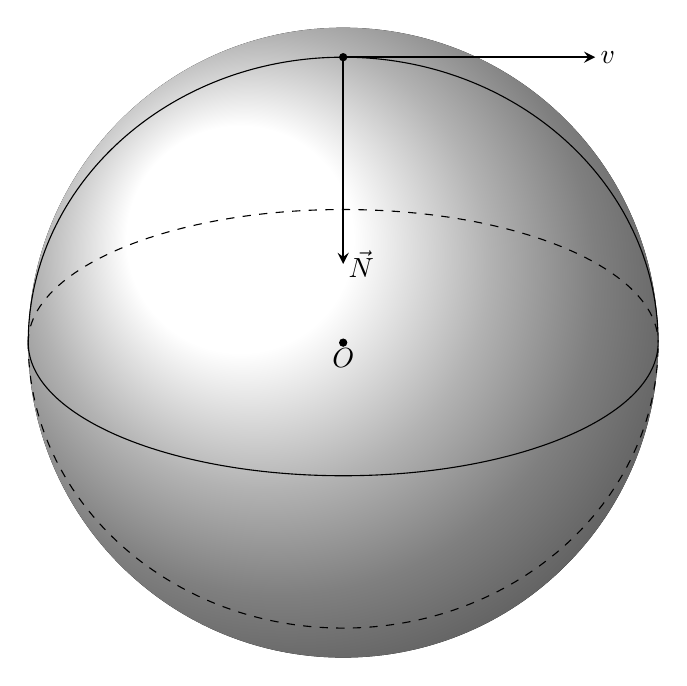
\begin{tikzpicture}[scale=2]%抄的知乎:https://zhuanlan.zhihu.com/p/494100190
                \pgfmathsetmacro{\R}{2};
                \pgfmathsetmacro{\AngleGamma}{25}
                \tikzset{%>=latex, % option for nice arrows
                    inner sep=0pt,%
                    outer sep=2pt,%
                     mark coordinate/.style=
                     {inner sep=0pt,outer sep=0pt,minimum size=3pt,
                    fill=black,circle}%
                        }
            \newcommand\LongitudePlane[3][current plane]{
            \tikzset{#1/.estyle={cm={cos(#3),sin(#3)*sin(#2),0,cos(#2),(0,0)}}}}
            \newcommand\DrawLongitude[3][\AngleGamma]{
            \LongitudePlane{#1}{#3}
            \tikzset{current plane/.prefix style={scale=#2}}
                             % angle of "visibility"
            \pgfmathsetmacro\angVis{atan(sin(#3)*cos(#1)/sin(#1))} %
            \draw[current plane,thin,black] 
            (\angVis:1) arc (\angVis:\angVis+180:1);
            \draw[current plane,thin,dashed] 
            (\angVis-180:1) arc (\angVis-180:\angVis:1);
            }
            \newcommand\LatitudePlane[3][current plane]{
  \pgfmathsetmacro\yshift{cos(#2)*sin(#3)}
  % 下面 cm 的最后一个参数不能出现乘法,所以定义了 yshift
  \tikzset{#1/.estyle={cm={cos(#3),0,0,cos(#3)*sin(#2),(0,\yshift)}}}
}
% 参数1:【可选】极点的倾斜角,默认 `\AngleGamma`
% 参数2:地球半径
% 参数3:维度(北正南负)
\newcommand\DrawLatitude[3][\AngleGamma]{
  \LatitudePlane{#1}{#3}
  \tikzset{current plane/.prefix style={scale=#2}}
  \pgfmathsetmacro\sinVis{sin(#3)/cos(#3)*sin(#1)/cos(#1)}
  % angle of "visibility"
  \pgfmathsetmacro\angVis{asin(min(1,max(\sinVis,-1)))}
  \draw[current plane,thin,black] (\angVis:1) arc (\angVis:-\angVis-180:1);
  \draw[current plane,thin,dashed] (180-\angVis:1) arc (180-\angVis:\angVis:1);
}        
	        {
                \fill[ball color=white!10] (0,0) circle (\R);
                \coordinate[mark coordinate] (N) at (0,{\R*cos(\AngleGamma)});
                \coordinate[mark coordinate] (O) at (0,0);
                \node[below] at (O) {\(O\)};
                \DrawLongitude{\R}{0};
                \DrawLatitude{\R}{0};
                \draw[->,>=stealth]
                (0,{\R*cos(\AngleGamma)})to({\R*0.8},{\R*cos(\AngleGamma)})
                node[right]{\(v\)};
                \draw[->,>=stealth]
                (0,{\R*cos(\AngleGamma)})to(0,{\R*0.25})
                node[right]{\(\vec{N}\)};
            }
            \end{tikzpicture}
        \end{center}
     \begin{example}\label{normal curvature-cylinder}
         Cylinder: \(x^2+y^2=1\).
     \end{example}
        \[\vec{N}:\text{ inner normal.}\]

        Let \(v_1\) be the unit normal along vertical lines.
        \(\implies\) normal section is just the line along \(v_1\) 
        \(\implies k_1=0\). Let \(v_2\) be the unit normal parallel
         to \(xy\) plane. \(\implies \) 
        normal section is a horizontal circle. \(\implies k_2=1\) (that is the 
        curvature of a circle). As we move the horizontal circle to the vertical line
        (\ie\ \(v_2\to v_1\)), the normal curvature is decreasing.
        
        \begin{center}
            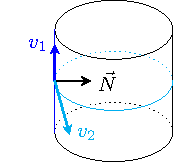
\includegraphics[scale=2]{picture/week7/cylinder7.pdf}
            \begin{comment}
            \tdplotsetmaincoords{30}{0}
            \begin{tikzpicture}[scale=3,tdplot_main_coords]
                \pgfmathsetmacro{\a}{0};
                \draw[smooth,variable=\x,domain=-180:180]
                plot ({cos(\x)},1,{sin(\x)});
                \draw[smooth,variable=\x,domain=\a:180+\a,dotted]
                plot ({cos(\x)},-1,{sin(\x)});
                \draw[smooth,variable=\x,domain=-180+\a:\a]
                plot ({cos(\x)},-1,{sin(\x)});
                \draw ({cos(\a)},-1,{sin(\a)})--({cos(\a)},1,{sin(\a)});
                \draw[blue] ({-cos(\a)},-1,{-sin(\a)})--({-cos(\a)},1,{-sin(\a)});
                \draw[smooth,variable=\x,domain=\a:180+\a,dotted,cyan]
                plot ({cos(\x)},0,{sin(\x)});
                \draw[smooth,variable=\x,domain=-180+\a:\a,cyan]
                plot ({cos(\x)},0,{sin(\x)});
            \draw[->,>=stealth,thick]
            ({-cos(\a)},0,{-sin(\a)})to({-cos(\a)*0.4},0,{-sin(\a)*0.4})
            node[right]{\(\vec{N}\)};
            \draw[->,>=stealth,thick,blue]
            ({-cos(\a)},0,{-sin(\a)})to({-cos(\a)},0.7,{-sin(\a)})
            node[left]{\(v_1\)};
            \draw[->,>=stealth,thick,cyan]
            ({-cos(\a)},0,{-sin(\a)})to
            (-0.75,0,-1.8)
            node[right]{\(v_2\)};
            \end{tikzpicture}
        \end{comment}
        \end{center}
        \begin{example}\label{normal curvature-catenoid}
            Catenoid: \(\varphi(u,v)=
            \left(c\cosh\frac{v}{c}\cos u,
            c\cosh\frac{v}{c}\sin u,v\right)\)
        \end{example}

        The normal section obtained by \(S\cap \Span\{v_1,\vec{N}\}\)
        is a catenary, with \(k_1<0\). The normal section obtained by 
        \(S\cap \Span\{v_2,\vec{N}\}\) is a circle, with \(k_2>0\).
        \begin{center}
        \begin{comment}
            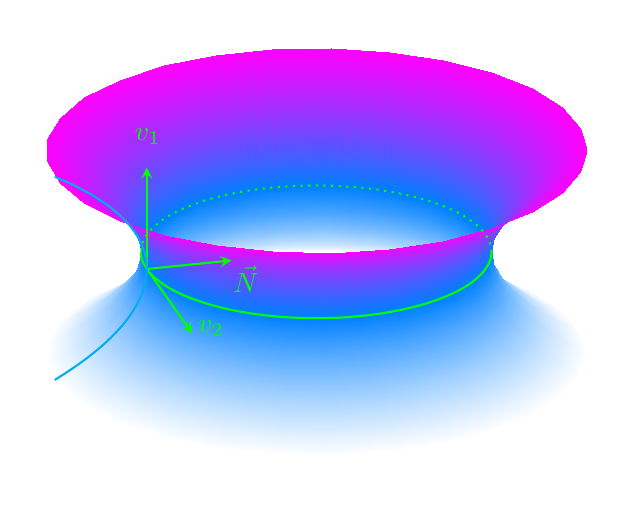
\begin{tikzpicture}
            \begin{axis}[xticklabels={,,},%不显示x坐标轴数字
                    yticklabels={,,},
                    zticklabels={,,},
                    axis line style={draw=none},%不显示坐标轴
                    tick style={draw=none},
                    colormap/cool,
                    view={0}{40}
                    ]
                \addplot3 [
                surf,
                shader=interp,
                z buffer=sort,
                domain=0:360, domain y=-1:1,
                samples=30, samples y=30,
                variable=\v, variable y=\u,
                %point meta=u
                ] ({cosh(u)*cos(v)},
                {cosh(u)*sin(v)},
                {u});
                \addplot3 [
                    green,
                    quiver={u=\thisrow{u},v=\thisrow{v},w=\thisrow{w}},
                    -stealth,
                ] table{
                    x y z u v w 
                    -0.96592582628 -0.2588190451 0 0 0 1 
                    -0.96592582628 -0.2588190451 0 0.2588190451 -0.96592582628 0 
                    -0.96592582628 -0.2588190451 0 0.48296291314 0.12940952255 0 
                };
                \addplot3 [
                    green,
                    domain=-180:0,
                    samples=40,
                    samples y=1%防止曲线闭合
                ]({cos(x)},{sin(x)},0);
                \addplot3 [
                    green,
                    dotted,
                    domain=0:180,
                    samples=40,
                    samples y=1%防止曲线闭合
                ]({cos(x)},{sin(x)},0);
                \addplot3 [
                    cyan,
                    domain=-1:1,
                    variable=\t,
                    samples=40,
                    samples y=1
                ]({cosh(t)*-0.96592582628},{cosh(t)*-0.2588190451},{t});
                \node[text=green] at (-0.96,-0.25,1.3) {\(v_1\)};
                \node[text=green] at (-0.60,-1.15,0) {\(v_2\)};
                \node[text=green] at (-0.4,-0.1,-0.2) {\(\vec{N}\)};
            \end{axis}
        \end{tikzpicture}
    \end{comment}
    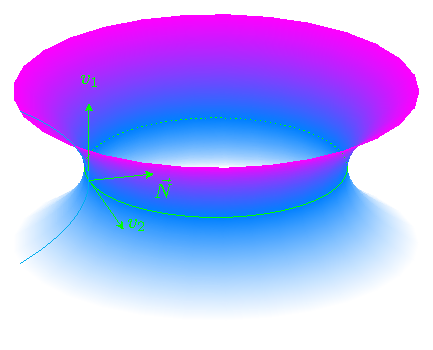
\includegraphics{picture/week7/catenoid-cool.pdf}
        \end{center}
    As you may notice, in \cref{normal curvature-sphere}, all 
    normal curvatures are the same at all points and along any 
    direction. In \cref{normal curvature-cylinder} and 
    \cref{normal curvature-catenoid}, at any point there are extremal
    directions at which the normal curvature achieves 
    the maximum and the minimum. Let's discuss more on these two special 
    normal curvatures.
\subsection{Principle curvature and principle direction}
Since \(\dd N_p\colon T_p S\to T_p S\) is linear and 
symmetric (self-adjoint), for any orthonormal basis {\(e_1,e_2\)},
\[
        \dd N_p\begin{pmatrix}
            e_1\\
            e_2
        \end{pmatrix}
        =\underbrace{\begin{pmatrix}
            a_{11}&a_{12}\\
            a_{21}&a_{22}
        \end{pmatrix}}_{symmetric}
        \begin{pmatrix}
            e_1\\
            e_2
        \end{pmatrix}
\]
\(\implies \exists\) an orthonormal basis {\(\tilde{e_1}
,\tilde{e_2}\)} of \(T_p S\) such that 
\[
        \dd{N}_p \begin{pmatrix}
            \tilde{e_1}\\
            \tilde{e_2}
        \end{pmatrix}
        =\begin{pmatrix}
            -k_1& 0\\
            0&-k_2
        \end{pmatrix}\begin{pmatrix}
            \tilde{e_1}\\
            \tilde{e_2}
        \end{pmatrix}
        \quad (k_1\ge k_2)
\]
\begin{definition}[Principle curvature and principle direction]
    \(k_1\) and \(k_2\) above are called the principle curvature
    and \(\tilde{e_1},\tilde{e_2}\) are called the principle
    directions at \(p\).
\end{definition}
\begin{remark}
    \(k_1\) and \(k_2\) are the maximum and minimum values of 
    the \engordnumber{2} fundamental form \(\II\) restricted on 
    the unit vectors of \(T_p S\).
\end{remark}
\begin{proof}
    \[
    \II\left(\tilde{e_1},\tilde{e_1}\right)=-\left\langle
        \dd N_p\left(\tilde{e_1}\right),\tilde{e_1}\right\rangle
        =\left\langle k_1 \tilde{e_1},\tilde{e_1}\right\rangle
        =k_1.
    \]
    Similarly, \(\II\left(\tilde{e_2},\tilde{e_2}\right)=k_2\).

    For any unit vector \(v\in T_p S\), \(v=
    v_1\tilde{e_1}+v_2\tilde{e_2}\), with \(|v|=1\).
    \begin{align*}
        \II(v,v)&=-\left\langle \dd N_p(v),v\right\rangle\\
        &=-\left\langle v_1 \dd N_p\left(\tilde{e_1}\right)
        +v_2\dd N_p\left(\tilde{e_2}\right),v_1\tilde{e_1}+v_2
        \tilde{e_2}\right\rangle\\
        &=k_1 v_1^2 +k_2 v_2^2=
        \begin{cases}
            k_1+(k_1-k_2)v_2^2\le k_1,\\
            (k_1-k_2)v_1^2+k_2\ge k_2.
        \end{cases}
    \end{align*}
    Hence, \(k_1\) and \(k_2\) are maximum and minimum values of normal
    curvature. Moreover, \(\forall\) unit vector \(v\in T_p S\) and 
    {\(e_1,e_2\)} the principle direction, we can write
    \[
        v=\cos \theta e_1+\sin\theta e_2,
    \]
    \[
        k_{\vb{n}}(v)=k_1 \cos^2\theta +k_2 \sin^2\theta.    
    \]
    The last is called ``Euler formula''.
\end{proof}
